\subsection{Topología ferroviaria original}

\lipsum[2]


\begin{figure}[H]
	\centering
	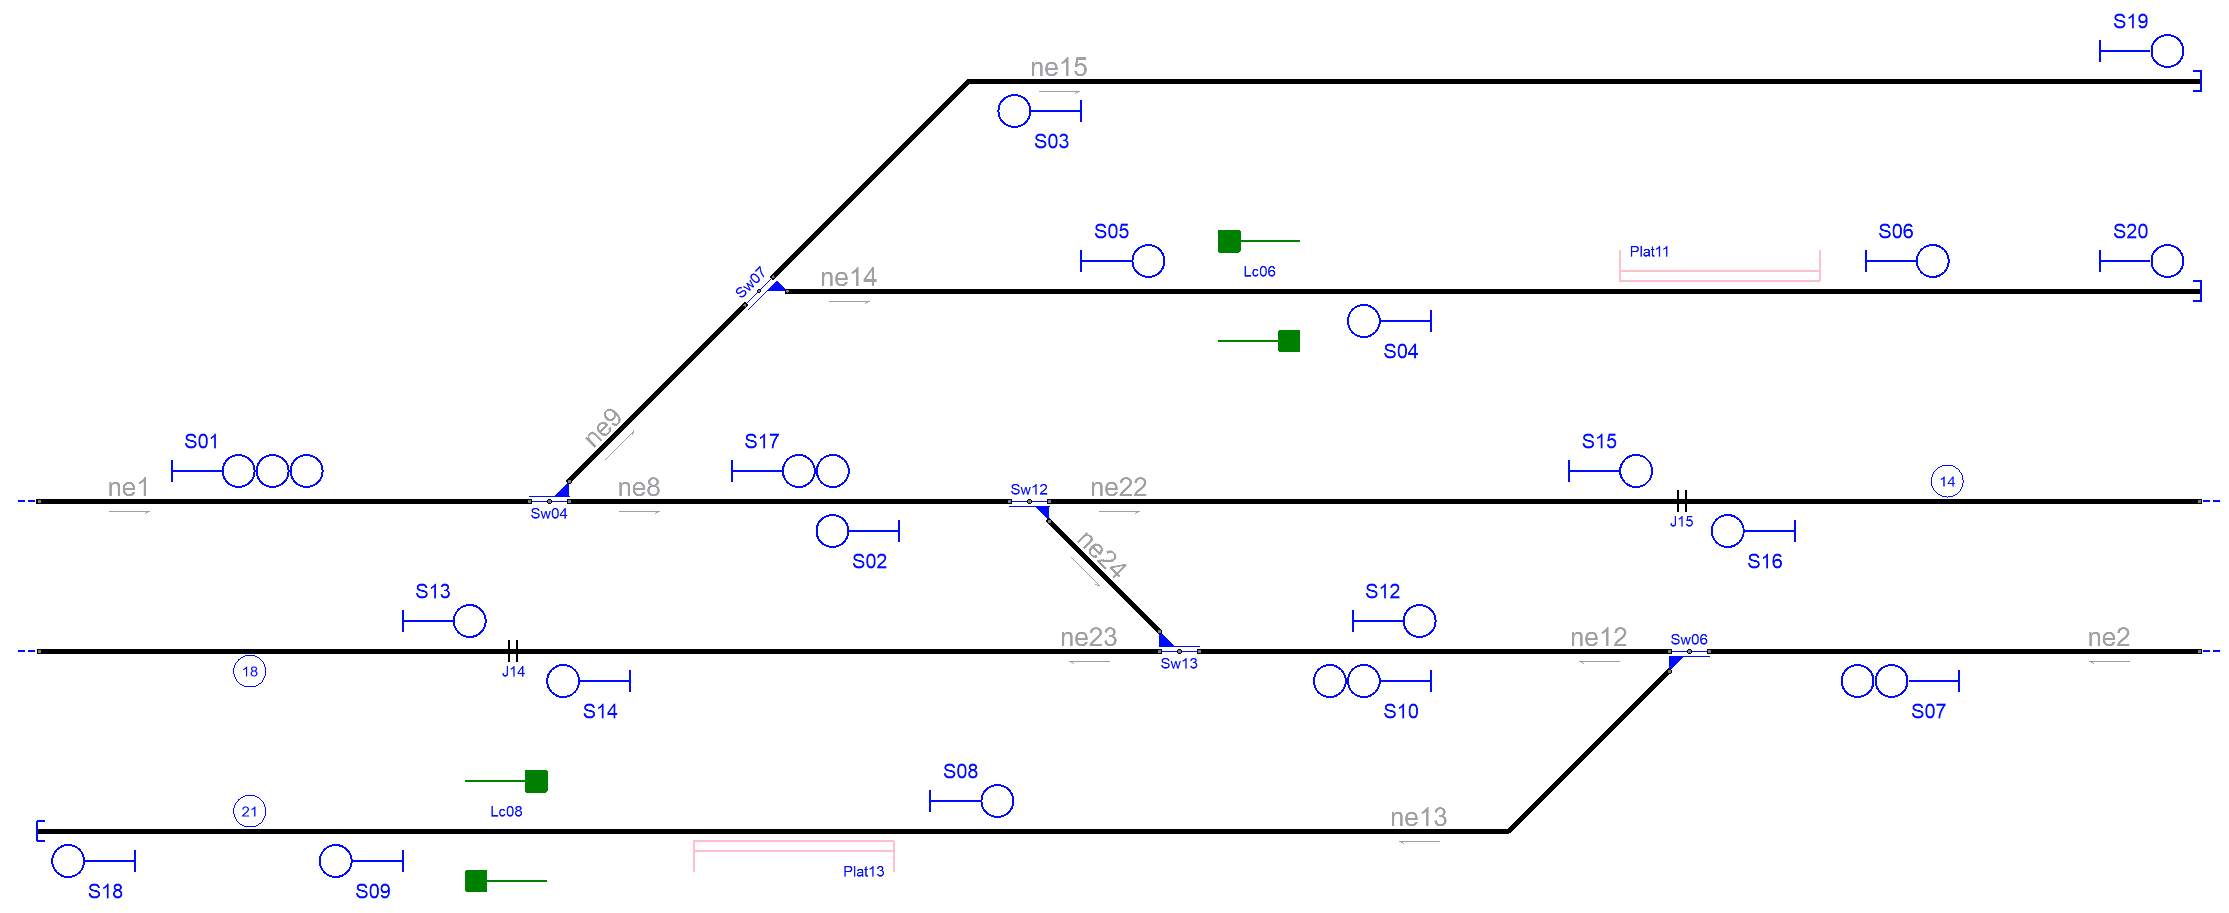
\includegraphics[width=1\textwidth]{resultados-obtenidos/ejemplo1/images/1_original.png}
	\centering\caption{Señalamiento original del ejemplo 1.}
	%\label{fig:LC_P2}
\end{figure}

\lipsum[2]

\begin{figure}[h]
	\centering
	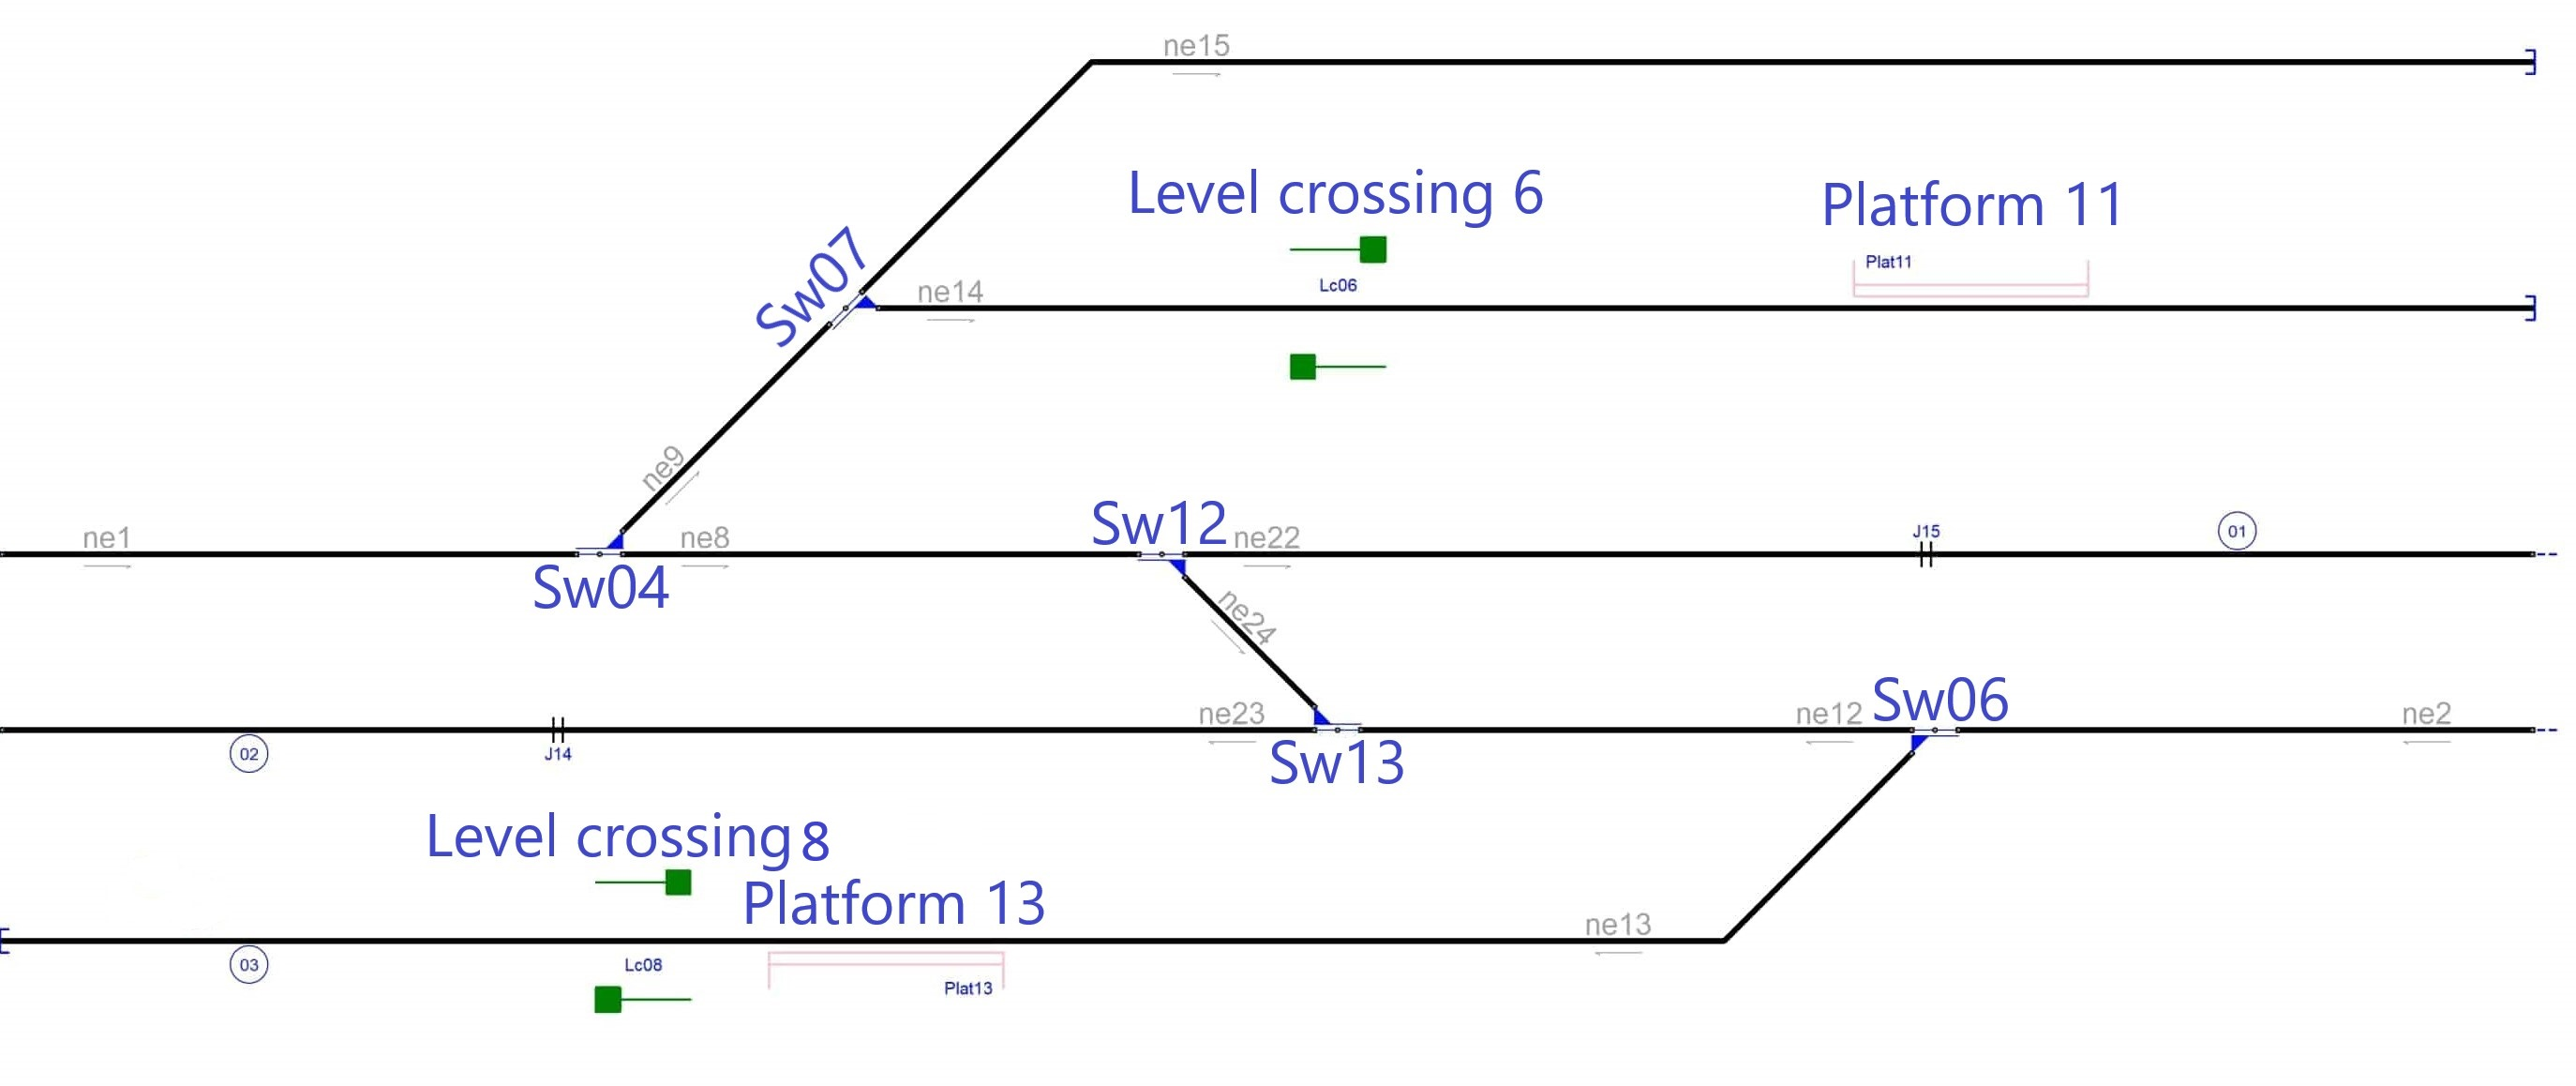
\includegraphics[width=1\textwidth]{resultados-obtenidos/ejemplo1/images/1_empty.png}
	\centering\caption{Topología ferroviaria del ejemplo 1 sin señalamiento.}
	%\label{fig:LC_P2}
\end{figure}

\lipsum[2]
